\uuid{KHHE}
\exo7id{2654}
\titre{exo7 2654}
\auteur{debievre}
\organisation{exo7}
\datecreate{2009-05-19}
\isIndication{false}
\isCorrection{false}
\chapitre{Fonction de plusieurs variables}
\sousChapitre{Extremums locaux}
\module{Analyse}
\niveau{L2}
\difficulte{}

\contenu{
\texte{
On consid\`ere la fonction 
$$f(x,y)=(1+2\cos^2(\pi x))(1-\exp(-y^2))+\sin(\pi x).$$
Son graphe est reproduit dans la figure ci-dessous.

\centerline{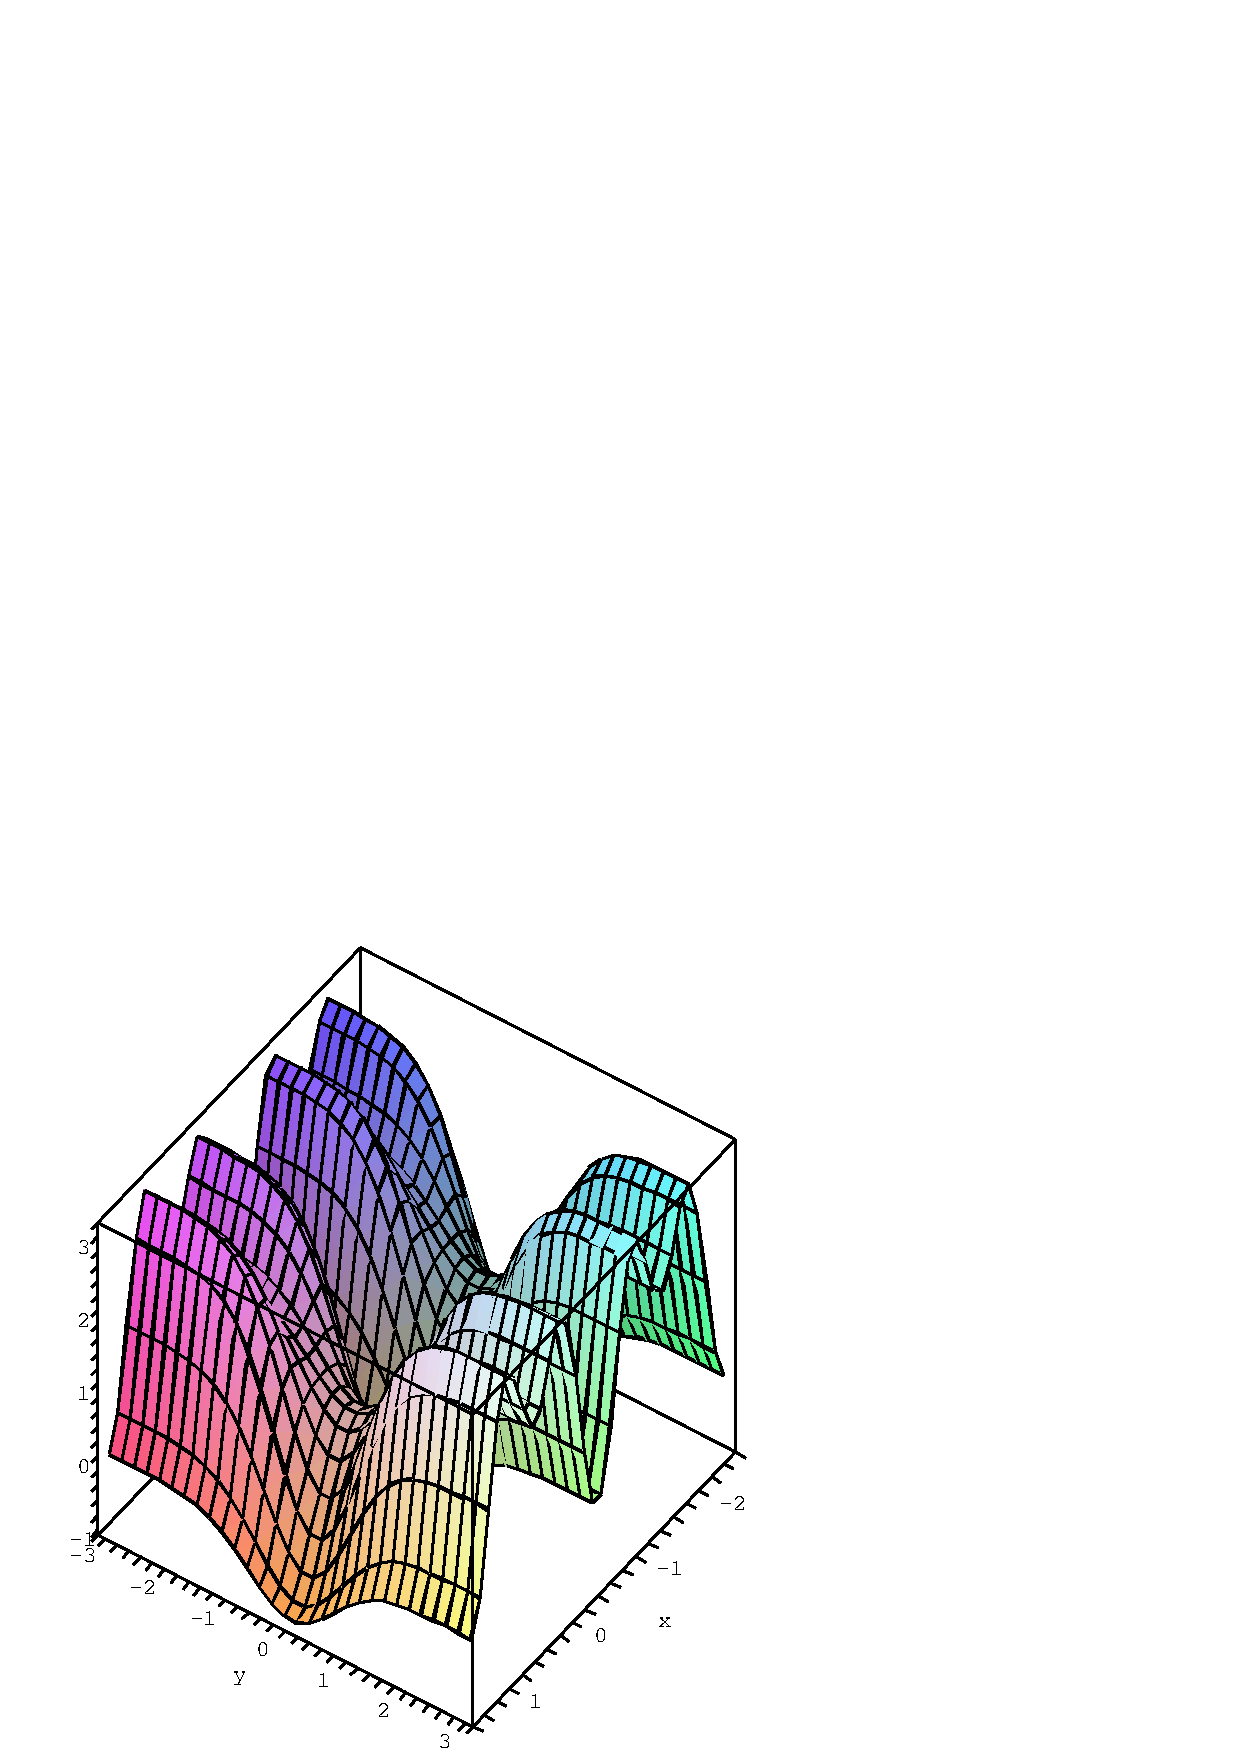
\includegraphics[height=8cm, keepaspectratio]{../images/pdf/KHHE-1.pdf}}
}
\begin{enumerate}
    \item \question{Trouver tous les points critiques de $f$ et d\'eterminer leur nature. Vos r\'esultats sont-ils compatibles avec le graphe de la fonction, reproduit ci-dessus?}
    \item \question{D\'eterminer l'\'equation du plan tangent au graphe de $f$ au point de coordonn\'ees $(1, 1, f(1,1))$. Tracer la droite d'intersection de ce plan avec le plan $xOy$.}
\end{enumerate}
}
